%! Author = leste
%! Date = 2026-09-14

% Preamble
\documentclass[%
reprint,
%superscriptaddress,
%groupedaddress,
%unsortedaddress,
%runinaddress,
%frontmatterverbose,
%preprint,
%preprintnumbers,
nofootinbib,
%nobibnotes,
%bibnotes,
 amsmath,amssymb,
 aps,
%pra,
%prb,
%rmp,
%prstab,
%prstper,
floatfix,
]{revtex4-2}

% Packages
\usepackage{graphicx}% Include figure files
\usepackage{dcolumn}% Align table columns on decimal point
\usepackage{bm}% bold math
\usepackage{siunitx}
\usepackage{booktabs}
\usepackage{derivative}
\usepackage{amsmath}


% Recommended options for physics papers:
\sisetup{
  separate-uncertainty = true, % Prints as (value ± uncertainty) unit instead of value(unc) unit
  multi-part-units = single    % Ensures units are not repeated, e.g., (1.23 ± 0.04) m instead of 1.23 m ± 0.04 m
}




%\usepackage[giveninits=true]{biblatex}
%\addbibresource{references.bib}


\newcommand{\UVic}{\affiliation{Department of Physics and Astronomy, University of Victoria, Canada}}
\newcommand{\dif}{\mathop{}\!\mathrm{d}}



% Document
\begin{document}

% \preprint{APS/123-QED}

\title{Experiment 32: Charge Oscillations and Energy Transfers in LRC Circuits}
%\title{Exploring the Focusing Mechanism of the NuMI Horn Magnets}%

\author{Mark Lester}\UVic

\date{\today}% It is always \today, today,
             %  but any date may be explicitly specified

\begin{abstract}
    This study's primary objective is to first, calculate critical values for resistance that lead to three defining
    configurations for a damped, discharging LRC circuit: normal, critical, and oscillatory damped cases;
    and second, demonstrate the
    relationship
    between
    electric and magnetic field
    energy exchange including losses from heat dissipation.
    Critical resistance values of the normal, critical, oscillatory cases were \qty{1133}{\ohm}, \qty{485}{\ohm}, and \qty{20}{\ohm}, respectively.
    Analysis on data collected by LabPro sensors and software demonstrated close agreement with the oscillatory
    case, with an experimental damped frequency of \qty{46}{\hertz} and a theoretical damped frequency of \qty{47.1(1.6)}{\hertz}.
    Energy analysis confirmed the continuous exchange between electric and magnetic field energy, however,
    erroneous conserved energy plots were produced from sensitive signal triggering in the software calibration.
    More appropriate trigger values and higher sample frequencies would
    help mitigate this problem and produce more accurate plots of conserved energy.
\end{abstract}


%\keywords{Suggested keywords}%Use showkeys class option if keyword
 %display desired
\maketitle

 %\tableofcontents
\section{Introduction}

Inductor, resistor, capacitor (LRC) circuits are a fundamental configuration of components that allows us to examine
the behaviour between electricity and magnetism.
This is because capacitors store energy in an electric field, and inductors store energy in its generated magnetic
field from the change in current, and a discharged circuit demonstrates the energy transfer between them.
Understanding LRC circuits is fundamental to modern electronics, and is responsible for radio
frequency communications from integrated
antennae in PCBs, motor drivers, and capacitive touch sensors, for example.

From Kirchoff's voltage law, the primary differential equation that models the discharge behaviour is

\begin{equation}\label{eq:diffyq}
L \odv[2]{i}{t} + R \odv{i}{t} + \frac{i}{C} = 0.
\end{equation}

Where $L$, $R$, $C$, $i$ are the inductance, system resistance, capacitance, and current, respectively.
The general solutions to this equation can be reduced to three configurations that display differing behaviour by
selecting
values for
$R$:
Normal ,
critical, and
oscillatory
damping; Eqs.~\eqref{eq:norm_damp}, ~\eqref{eq:crit_damp}, and \eqref{eq:osc_damp}, respectively.

\begin{equation}\label{eq:norm_damp}
\left( \frac{R}{2 L}\right)^2 - \frac{1}{L C} > 0
\end{equation}

\begin{equation}\label{eq:crit_damp}
\left( \frac{R}{2 L}\right)^2 - \frac{1}{L C} = 0
\end{equation}

\begin{equation}\label{eq:osc_damp}
\left( \frac{R}{2 L}\right)^2 - \frac{1}{L C} < 0
\end{equation}

For the critically damped case, theoretical predictions can be made on the voltage signals.
The theoretical equations for current and voltage are given by the following:

\begin{equation}
i = \frac{V_0}{L} t e^{- \frac{R}{2 L}t}.\label{eq:i_theo}
\end{equation}

\begin{equation}\label{eq:vl_theo}
V_L = -V_0 \left(1 - \frac{R}{2 L} t\right) e^{- \frac{R}{2 L}t}.
\end{equation}

\begin{equation}\label{eq:vc_theo}
V_C = V_0 \left(1 + \frac{2}{R C} t\right) e^{- \frac{R}{2 L}t}.
\end{equation}

$V_0$, $V_L$, $V_C$ are the values for the steady state voltage, inductor, capacitor electric potentials,
respectively.
For the oscillatory case, the theoretical frequency of oscillation is given by

\begin{equation}\label{eq:freq}
j \omega = \sqrt{\frac{R^2}{4 L^2} - \frac{1}{L C}}.
\end{equation}

The energetics of the system can be calculated using potential energy equations:

\begin{equation}\label{eq:el}
    E_L = \frac{1}{2} Li^2
\end{equation}

\begin{equation}\label{eq:ec}
    E_C = \frac{1}{2} C V_C^2
\end{equation}

And the thermal heat energy dissipated is calculated using

\begin{equation}\label{eq:heat}
    E_H = \int_{t_n}^{t_{n+\Delta t}} Ri^2 \dif t \approx R i_{AV}^2 \Delta t,
\end{equation}

where $\Delta t$ is the evaluated time step between samples, and $i_{AV}$ is the average current over the time
interval given by

\begin{equation}\label{eq:i_av}
    i_{AV} = \frac{V_R}{R_{res}}.
\end{equation}


\section{Apparatus}

Equipment: Vernier LabPro sensor interface, LabPro software, 4000 turn inductor, electrolytic capacitor, decade resistance box,
differential voltage probes, Instek GFG-8219A function generator, Wavetek LCR55 digital multimeter with alligator
clip probes, banana plug cables.

\begin{figure}[htb]
    \centering
    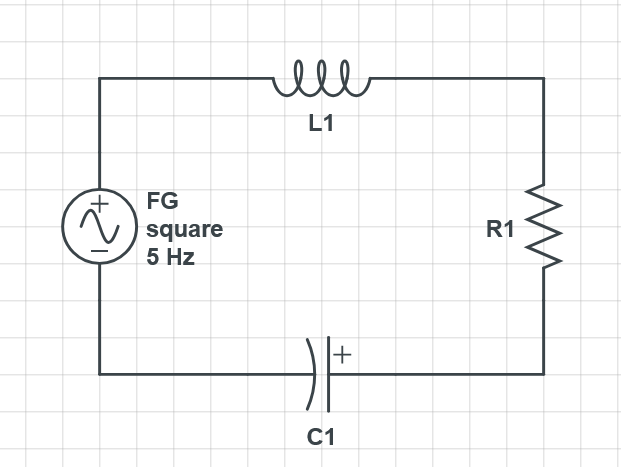
\includegraphics[width=\linewidth,height=0.35\textheight,keepaspectratio]{fig/circuit_diag}
    \caption{LRC circuit. Probes were connected across L, R, C components to measure voltage in the LabPro Software.}
    \label{fig:diag}
\end{figure}
\section{Procedure}

The experimental apparatus and procedure followed the standard method
    outlined in the University of Victoria PHYS 326 laboratory manual~\cite{phys326}.

A circuit comprised of an inductor, resistor, and capacitor (LRC circuit) was assembled in series connected to a
function generator.
Measurements of the inductance, resistance, and capacitance were taken of each component with the digital multimeter
before connecting the circuit.
Table~\ref{tab:params} provides a list of measurements taken.
Uncertainty was calculated using the digital multimeter's spec sheet, including the range's relative and per digit
uncertainty.

\begin{table}[htbp]
\caption{Experimental Parameters}
\begin{tabular}{lrrr}
\toprule
{Quantity} & {Reading} \\
\midrule
$R_L$, Inductor resistance & \qty{109.4(1.3)}{\ohm} \\
L, Inductance & \qty{1.044(0.072)}{\henry} \\
C, Capacitance & \qty{10.07(0.21)}{\micro\farad}\\
$R_{FG}$, function generator resistance & \qty{50.00(0.25)}{\ohm} \\
$R_{res}$, normal & \qty{1133}{\ohm} \\
$R_{res}$, critical & \qty{485}{\ohm} \\
$R_{res}$, oscillatory & \qty{20}{\ohm} \\
\bottomrule
\end{tabular}\label{tab:params}
\end{table}

The function generator was configured to output a 5 Hz square wave signal to act as a continuous
switch for the LRC circuit to quickly cycle between charge and discharge.
The function generator offset was manually adjusted such that the ``ON'' and ``OFF'' settings were set to 3.86 V and
0 V, respectively.
Vernier differential probes were connected to the LabPro sensor interface and the LabPro software was calibrated to
take voltage readings at 3000 samples per second.

Before each data were collected, care was taken to ensure the probes were both physically shorted and zeroed in the
software to mitigate charge buildup that might offset the readings.
A preliminary test case was done to adjust the maximum recording time so that the majority of the discharge cycle
was captured without extending to the charging cycle.
The maximum time was set to 0.09 seconds, which appeared to consistently capture the whole event.
Resistor values were calculated to define damped, critically damped, and oscillatory behaviour for the LRC circuit.
The critical resistance value for the damped case was set to be double that of the critically damped case to ensure
signal behaviour between the two cases were appropriately different.
Once the decade resistance box was set using the dials, a discharge cycle was recorded via a voltage trigger and values
for inductor,
resistor, and
capacitor voltages produced.
This was done a total of three times, completed once for each damped, critically damped, and oscillatory case.


\section{Results}

\begin{figure}[htb]
    \centering
    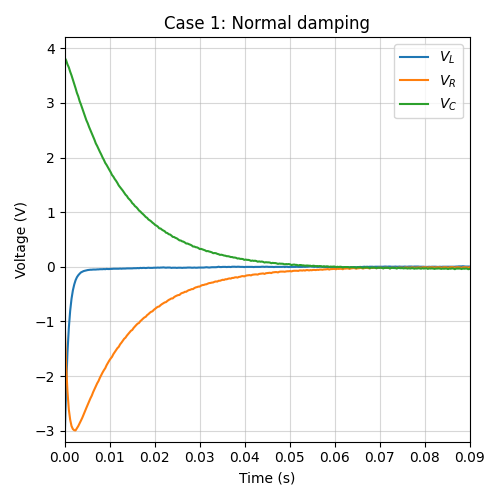
\includegraphics[width=\linewidth]{fig/case1_normal_damping}
    \caption{Signals showing normal damping behaviour.}\label{fig:normal_damp}
\end{figure}

In Figure~\ref{fig:normal_damp}, the circuit is normally damped such that the components discharge gradually over
the cycle to zero volts without oscillating.
The resistance value chosen here was calculated using double the critical system resistance found in Eq.~\eqref{eq:crit_damp}, which ended up being \qty{1133}{\ohm}.

\begin{figure}[htb]
    \centering
    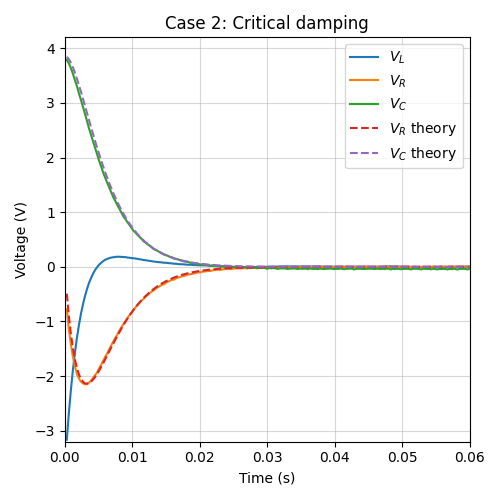
\includegraphics[width=\linewidth]{fig/case2_crit_damping}
    \caption{Signals showing critical damping behaviour.}\label{fig:crit_damp}
\end{figure}

In Figure~\ref{fig:crit_damp}, the resistance chosen using Eq.~\eqref{eq:crit_damp} was \qty{485}{\ohm}.
Notice the quicker time to reach zero volts compared with case 1.

\begin{figure}[htb]
    \centering
    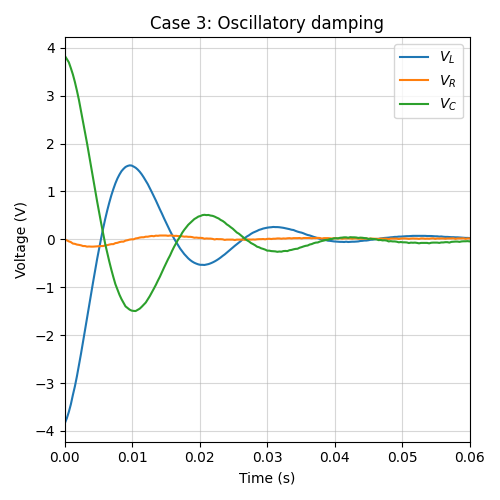
\includegraphics[width=\linewidth]{fig/case3_oscillatory_damping}
    \caption{Signals showing oscillatory damping.}\label{fig:osc_damp}
\end{figure}

Figure~\ref{fig:osc_damp} shows that at selected resistance \qty{20}{\ohm}, the behaviour turned oscillatory.
Since the resistance was much lower, more of the electric potential remained within the inductor and capacitor during
the whole discharge cycle.

\begin{figure}[htb]
    \centering
    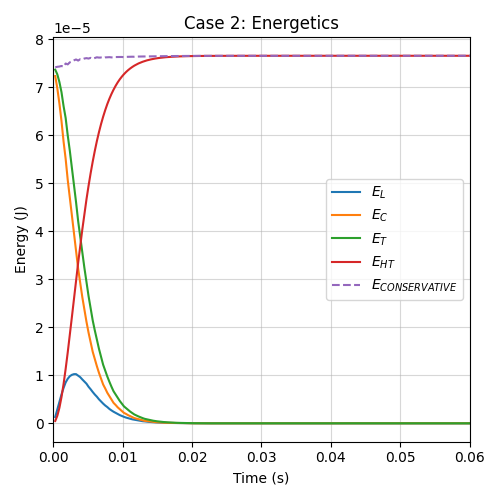
\includegraphics[width=\linewidth]{fig/case2_energetics}
    \caption{Critically damped energetics}\label{fig:case2_energy}
\end{figure}

\begin{figure}[htb]
    \centering
    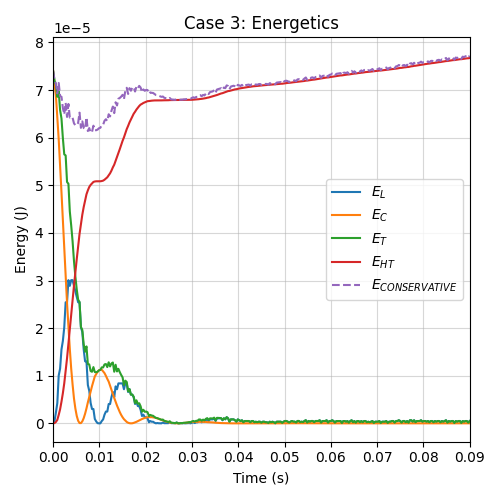
\includegraphics[width=\linewidth]{fig/case3_energetics}
    \caption{Oscillatory energetics}\label{fig:case3_energy}
\end{figure}

Figures~\ref{fig:case2_energy} and~\ref{fig:case3_energy} demonstrate the energetics of the system in critically
damped and oscillatory cases.
In both figures, it shows that once the discharge is initiated, the stored energy transfers between the
electric and magnetic fields of the circuit.
As $E_T$ decreases, the accumulated dissipated thermal energy, $E_{HT}$,
rises due
to joule heating.

\begin{table}[htbp]
    \caption{Oscillation Frequency}
    \begin{tabular}{lrrl}
        \toprule
        {Quantity}                      & {Value}           & {Units} \\
        \midrule
        Experimental frequency          & 46                & Hz      \\
        Theoretical natural frequency   & \qty{49.1(1.8)}{} & Hz      \\
        Theoretical frequency incl. $R$ & \qty{47.1(1.6)}{} & Hz      \\
        \bottomrule
    \end{tabular}\label{tab:osc_freq}
\end{table}

The oscillation frequency results are listed in Table~\ref{tab:osc_freq}.
Experimental frequency was determined by measuring the peak-peak time and dividing by the period.
Theoretical values were calculated using Eq.~\eqref{eq:freq}.
The theoretical natural frequency is close, but not quite consistent with the determined value, however, the
theoretical frequency taking into account $R$ is consistent.
This suggests the small damping resistance produces a system frequency lower than the natural frequency.
Note: Uncertainties in values were calculated using the aid of the \textit{uncertainties} python package.



\section{Discussion}

Figures~\ref{fig:normal_damp},~\ref{fig:crit_damp}, and~\ref{fig:osc_damp} show the voltage signals of the components
agree with the theoretical predictions.
The critically damped system discharges quicker than the normally damped configuration, and the oscillatory system
shows the electric potential transferring between the magnetic and electric fields.
Furthermore, the theoretical models for $V_R$ and $V_C$ align almost exactly to the recorded experimental signals.
Small differences between the experimental and theoretical results here can be explained by the resolution of the
evaluated time step, $\Delta t$.
As $\Delta t$ converges to zero, the difference between the theory and experiment would decrease.
The $V_R$ and $V_C$ signals attenuate much faster in the critically damped case.
This is due to the current decreasing faster as a result of the reduced resistance in the circuit.

However, in examining the energetics in Figures~\ref{fig:case2_energy} and~\ref{fig:case3_energy}, the conserved energy
unexpectedly rose above the initial total energy.
This suggests the sum of cumulative heat dissipation energy and total energy did not agree with theoretical predictions.
Since no external energy sources existed in the circuit, the increase in energy can be explained by a few
contributing factors.
In the oscillatory case, the energy transfer between electric and magnetic fields decreased in magnitude over time but
never reached
zero during the cycle.
In addition, the accumulated heat dissipation, $E_{HT}$, increased rapidly and unexpectedly rose higher than the
initial energy of the system.
This can be explained by the fact that the whole cycle was not captured from initial discharge, but indeed
began slightly after due to the software's trigger settings.


$E_T$ and $E_{HT}$ show to have correlated signals in both cases.
When $E_T$ drops, $E_{HT}$ rises, and when $E_T$ begins to plateau, so does $E_{HT}$.
This is because the total energy of the components transferred into the current through the system, thus resulting
in joule heating.
In Case 2, $E_{HT}$ plateaus quickly because current rapidly attenuates from critically damped discharge.
In Case 3, $E_{HT}$ gradually plateaus because the induced current from oscillations takes longer to attenuate.

Also, though a small contribution, the model does not take into account the thermal heat dissipated through the wires
connecting the circuit, only that of the system impedance of the individual components.
As temperatures change, so do the internal resistances of the components, further affecting the
calculated result due to changing current flow.

Analysing the frequency response of the oscillatory case, we found that the experimentally determined frequency was
consistent with the theoretical frequency taking into account the system resistance, $R$.
The theoretical natural frequency of the system was found to be slightly higher and just outside
consistency margins.
This suggests the damped frequency is slightly lower than the natural frequency of the system due to the
contributing damping resistance, $R$.


\section{Conclusion}

From our experimental analysis, the transient response of the LRC circuit under normal, critical, and oscillatory
damped configurations demonstrated the relationship between electric and magnetic fields during a discharge event.
The electric potential clearly showed that energy was exchanged back and forth between the components, and the
experimental
signals strongly agreed with the theoretical prediction curves.
In addition, the frequency calculations were consistent with experimental observations.

The energetics plots
demonstrated an unexpected increase in conserved energy, but this was explained by the data being captured too far
ahead
of the initial discharge event.
This erroneous reduction in the initial total energy stored in the
circuit led to a pseudo upward trend in the conserved energy.
By adjusting the trigger settings to be more sensitive to the falling edge of the signal, a full capture of the
discharge cycle, from fully
charged to
fully discharged, would
have shown a higher initial total
energy, and thus shown the conservative energy to gradually decrease.



\clearpage            % Flushes two-column floats and starts a fresh page
\onecolumngrid        % Switches REVTeX to full page width

\appendix
\section{Sample Calculations}

Critical resistance values were calculated via

$$
\begin{aligned}
R_{calc} &= 2 \cdot \sqrt{ \left( \frac{ L }{ C } \right)} \\&= 2 \cdot \sqrt{ \left( \frac{ \left(1.044 \pm 0.072\right) \times 10^{0} }{ \left(1.007 \pm 0.021\right) \times 10^{-5} } \right)} \\&= \qty{644(23)}{\ohm} \\
\\
R_{res} &= R_{calc} - R_{L} - R_{fg} \\&= \left(6.440 \pm 0.233\right) \times 10^{2} - \left(1.094 \pm 0.013\right) \times 10^{2} - \left(5.000 \pm 0.025\right) \times 10^{1} \\&= \qty{484(23)}{\ohm}  \\
\end{aligned}
$$

The theoretical natural frequency is
$$
\begin{aligned}
    f_{theo} &= \left( \frac{ 1 }{ 2 \cdot \pi } \right) \cdot \sqrt{\left(\frac{ 1 }{ L \cdot C } \right)} \\
    &= \left( \frac{ 1 }{ 2 \cdot \pi } \right) \cdot \sqrt {\left(
                                                                 \frac{ 1 }{ \left(1.044 \pm 0.072\right)
                                                                 \cdot \left(1.007 \pm 0.021\right) \times 10^{-5} }
    \right)} \\
    &= \qty{49.09(1.77)}{\hertz}
\end{aligned}
$$

Theoretical damped frequency is

$$
\begin{aligned}
f_{theo} &= \left( \frac{ 1 }{ 2 \cdot \pi } \right) \cdot \sqrt { \left( \frac{ 1 }{ L \cdot C } \right) - \left( \frac{ \mathrm{R} }{ 2 \cdot L } \right) ^{ 2 } } \\&= \left( \frac{ 1 }{ 2 \cdot 3.142 \times 10 ^ {0} } \right) \cdot \sqrt { \left( \frac{ 1 }{ \left(1.044 \pm 0.072\right) \times 10^{0} \cdot \left(1.007 \pm 0.021\right) \times 10^{-5} } \right) - \left( \frac{ \left(1.794 \pm 0.013\right) \times 10^{2} }{ 2 \cdot \left(1.044 \pm 0.072\right) \times 10^{0} } \right) ^{ 2 } } \\
&= \qty{47.14(1.59)}{\hertz}\\
\end{aligned}
$$

Average current is calculated by

$$
\begin{aligned}
i_{av} &= \frac{ V_{R} }{ R_{res} } \\
&= \frac{-7.751 \times 10 ^ {-1}}{-1.144 \times 10 ^ {0}} \\
&= \qty{-1.598e-3}{\ampere}
\end{aligned}
$$

Theoretical $V_R$ is

$$
\begin{aligned}
V_{R} &= \left( \frac{ \left( - V_{0} \right) }{ L } \right) \cdot t \cdot \exp \left( \left( - R \right) \cdot \frac{ t }{ 2 \cdot L } \right) \cdot R_{res} \\&= \left( \frac{ \left( - 3.860 \times 10 ^ {0} \right) }{ 1.044 \times 10 ^ {0} } \right) \cdot 6.000 \times 10 ^ {-4} \cdot \exp \left( \left( - 6.444 \times 10 ^ {2} \right) \cdot \frac{ 6.000 \times 10 ^ {-4} }{ 2 \cdot 1.044 \times 10 ^ {0} } \right) \cdot 4.850 \times 10 ^ {2} \\&= -8.940 \times 10 ^ {-1} \mathrm{V}  \\
\end{aligned}
$$

Stored inductor energy is

$$
\begin{aligned}
E_{L} &= 0.5 \cdot L \cdot \left( i_{av} \right) ^{ 2 }  = 0.5 \cdot 1.044 \times 10 ^ {0} \cdot \left( -2.360 \times 10 ^ {-3} \right) ^{ 2 } &= 2.907 \times 10 ^ {-6} \mathrm{J}
\end{aligned}
$$

\section{Source code and raw data}

The source code and raw data may be found it the public git repository:

\url{https://github.com/trolley-lorry/phys_bsc_data.git}.


\bibliography{references}
\bibliographystyle{apsrev4-2}
%\bibliographystyle{plain}




\end{document}